\documentclass[12pt, letterpaper]{article}
\usepackage[utf8]{inputenc}
\usepackage{graphicx}
\usepackage{hyperref}

%opening
\title{Bloom-Filter}
\author{DE SOUSA Benoît und SCHNEIDER Eloi}

\begin{document}

\maketitle

\section{Idee des Bloom-Filters}
Heutzutage gibt es viele Datenbanken und sehr oft wird nachgesehen, ob ein Wort (in unserem Fall) bereits in der Datenbank ist. Diesen Abfragen werden als vergleichbare Algorithmen bezeichnet, dh sie vergleichen das getestete Wort mit jedem Wort in der Datenbank. Aber solche Anfragen benötigten sehr viel Speicherplatz.\\
1970 fand Burton Howard Bloom eine Lösung. Er entwickelte den Bloom-Filter. Es ist eine probabilistische Datenstruktur.\\
Seine Idee war wie folgt. Er wollte die Abfragen in der Datenbank mit einem Bloom-Filter reduzieren, der vor der Datenbank platziert wird.\\
Er besteht aus einem m-stelligen Bit-Array (das am Anfang mit Nullen gefüllt ist) und aus k verschiedenen Hashfunktionen mit einem Wertebereich von 0 bis m-1 (m und k sind natürliche Zahlen mit k grösser als 0). Die Wörter, die in der Datenbank gespeichert werden, treten zuerst in den Bloom-Filter. Die k Hashfunktionen verarbeiten diesen Wörter und geben als Ergebnis k Zahlen zwischen 0 und m-1 zurück. Diese Zahlen stellen alle Bit in dem m-stelligen Bit-Array dar, die auf 1 eingesetzt werden müssen.\\
Die Abfrage können dann beginnen. Der Bloom-Filter erhält zuerst die Abfragen. Das getestete Wort folgt dem gleichen Prozess wie die anderen Wörter. Hier wieder werden Zahlen zwischen 0 und m-1 zurückgegeben. Der Bloom-Filter wird diese Zahlen/Positionen mit seinem Bit-Array vergleichen. Wenn es Unterschiede gibt, dann befindet sich das getestete Wort sicherlich nicht in der Datenbank. Andernfalls ist das getestete Wort nicht unbedingt in der Datenbank vorhanden. Es ist möglich, dass die durch die Hashfunktionen des getesteten Wortes erzeugten Positionen in die Positionen 1 fallen. Solche Fehler werden als falsch positive Ergebnisse bezeichnet.\\
Um einen Bloom-Filter verwenden zu können, ist es wichtig, die Anzahl der gespeicherten n Wörter und die Fehlerwahrscheinlichkeit p zu kennen, dh die Wahrscheinlichkeit, dass ein falsch positive Ergebnisse vorliegt. Die Werte von n und p werden verwendet, um die Länge des Bit-Arrays m und die Anzahl der Hashfunktionen k zu ermitteln.

\section{Vorteilen}

Ein Bloom-Filter hat zwei grossen Vorteilen.

Einerseits gibt es den Vorteil des Speichers, d.h. ein Bloom-Filter nimmt sehr wenig Speicherplatz ein. Dieser Speicherplatz ist auch konstant. Seine Größe ist unabhängig von der Anzahl der enthaltenen Elemente.

Andererseits gibt es den Vorteil der Zeit. Ein Bloom-Filter vermeidet unnötige Aufrufe einer sehr großen Datenbank und überprüft sofort, ob das gesuchte Objekt nicht vorhanden ist.\\

Der Bloom-Filter hat auch die Eigenschaft, dass die Zeit, die benötigt wird, um Elemente hinzuzufügen oder zu überprüfen, ob sich ein Element in der Datenbank befindet, eine feste Konstante ist, die Komplexität ist O(k) (k ist die Anzahl der Hashfunktionen), völlig unabhängig von der Anzahl der Elemente in der Datenbank.

\section{Nachteilen}

Aber ein solcher Filter ist nicht perfekt. Er hat auch einigen Nachteilen.

Zuerst kann den Filter falsch positive Ergebnisse als Antwort zurückgeben. Falsch positive Ergebnisse sind Objekte, die sich nicht in der Datenbank befinden, aber dennoch vom Filter in der Datenbank gesehen werden, da die Hashfunktionen immer an eine Stelle zurückgegeben werden, an der es eine 1 gab. Danach wird eine unnötige Suche in der gesamten Datenbank durchgeführt und schließlich eine negative Antwort erhalten.\\
Dieses Problem der Anzahl der falsch positiven Ergebnisse hängt von der Anzahl der Wörter der Datenbank ab. Je mehr Wörter in der Datenbank vorhanden sind, desto mehr falsch positive Ergebnisse können auftreten. Dennoch ist es wichtig zu beachten, dass es möglich ist, bei der Erstellung des Filters eine Wahrscheinlichkeit für falsch positive Ergebnisse zu definieren und so das Risiko, diese zu erhalten, zu reduzieren.\\

Zweitens ist das Entfernen eines Elements unmöglich, weil das Auftreten von falsch negativen Ergebnissen nicht erlaubt ist.

\section{Beispiel aus der Praxis}

Der Bloom-Filter hat in der Praxis viele Anwendungen. Eine dieser Anwendungen ist das URL-Testen von gefährlichen Websites. Es ist diese Funktion, die die Webbrowser Google verwendet. Tatsächlich erlaubt der Bloom-Filter, die URLs aller Websites zu testen, indem er sie mit ihrer gefährlichen Website-Datenbank vergleicht.\\
Die Größe eines solchen Filters ist sehr klein im Vergleich zu der Größe, die durch den Vergleichstest einer Website in der Datenbank dargestellt würde, was diesen Filter viel vorteilhafter macht.

\section{Test unserer Datenstruktur}

Unser erster Test war die Erstellung eines Filters vor einer Wahrscheinlichkeit p von 3\%. Danach haben wir einige Tests gemacht.\\
Von 1) zu 4) sind das Wörter, die sich in Wörter.txt befinden. Die Antwort ist true. Also ist das in Ordnung.\\
Von 5) bis 6) sind das Wörter, die nicht in Wörter.txt enthalten sind und gut erkannt wurden.\\
Von 7) bis 8) sind das Wörter, die nicht sich in Wörter.txt enthalten sind und die falsch erkannt wurden. Es sind falsch positiven Ergebnisse. \\ \\
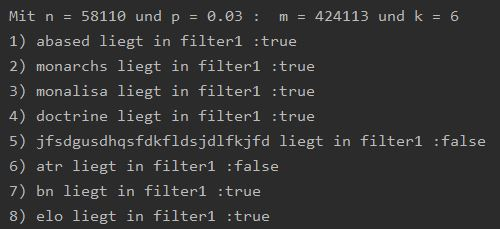
\includegraphics{../Image/filter1}\\ \\
Wir haben diesen Test noch einmal durchgeführt. Aber diesmal wurde p auf 1\% reduziert.\\
Der Unterschied liegt in den falsch positiven Ergebnissen. Er zeigt uns, dass je kleiner p ist, desto kleiner ist die Anzahl der falsch positiven Ergebnisse.\\ \\
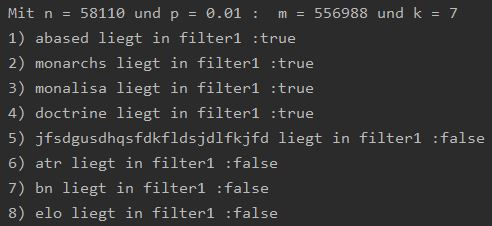
\includegraphics{../Image/filter2}

\section{Quellen}
Bloom-Filter, wikipedia \url{https://en.wikipedia.org/wiki/Bloom\_filter}

\end{document}
